%\documentclass[a4paper,12pt,oneside,openright,final]{memoir} %twocolumn,
\documentclass[a4paper,12pt,oneside,openright]{memoir}

\let\footruleskip\undefined
\usepackage[utf8]{inputenc}
\usepackage[english]{babel}
\usepackage{etex}
\usepackage{times}
\DisemulatePackage{setspace}
\usepackage{setspace}
\usepackage{amssymb}
\usepackage{amsfonts}

\usepackage{graphicx}
\usepackage[printwatermark]{xwatermark}
% uncomment for watermarks
%\newwatermark[allpages,color=red!10,angle=45,scale=5,xpos=-15,ypos=30]{DRAFT}

\usepackage{alltt}
\usepackage{moreverb}
%for more info on hyperref package see http://en.wikibooks.org/wiki/LaTeX/Packages/Hyperref
\usepackage[pdftex,colorlinks=true,linkcolor=blue, citecolor=magenta]{hyperref}
\usepackage{eso-pic}
\usepackage{transparent}
\setlength{\columnsep}{3em}

\usepackage{tcolorbox}
\usepackage{listings}
\definecolor{codebgcolor}{HTML}{6E84D6}  
\definecolor{codefgcolor}{HTML}{000000}% 071D70
\definecolor{basiccolor}{HTML}{000000}%1435AD
\definecolor{stringcolor}{HTML}{050505}% 2C3E82
\definecolor{highlight}{HTML}{FFB100}
\definecolor{annotationbgcolor}{HTML}{FFD473}

\usepackage{wrapfig}
\usepackage{caption}
\usepackage{subcaption}
\usepackage{alltt}
\usepackage{moreverb}
% tikz related packages to provide scalable graphics 
\usepackage{tikz}
\usetikzlibrary{calc,mindmap,backgrounds,positioning,arrows,shapes,shapes.arrows,shapes.misc,automata,petri,patterns,scopes,chains,matrix,decorations.pathmorphing,shadows,calc}

\usepackage{geometry}
\geometry{hmargin={15mm,15mm},vmargin={15mm,20mm}}

\usepackage[pages=some]{background}

\backgroundsetup{
  scale=1.2,
  angle=0,
  opacity=0.4,
  contents={
    
\includegraphics[width=1.1\paperwidth,height=1.1\paperheight, keepaspectratio]{images/00-background.png}} 
}


%%%%%%%%%%%%% copyright %%%%%%%%%%%%%%
\title{Application security in TG applications}
\author{Fielden Management Services Pty. Ltd.}
\date{}
\usepackage{hyperxmp}
\hypersetup{
    pdftitle={Application security in TG applications},
    pdfauthor={Fielden Management Services Pty. Ltd.},
    pdfsubject={An overview of key principles and approaches to security in TG applications.},
    pdfcopyright={Copyright (C) 2019 by Fielden Management Services Pty. Ltd.  All rights reserved.}
}

\usepackage{xcolor}
\makeevenhead{headings}%
    {\thepage}{}{\slshape\bookname~\thebook\qquad\partname~\thepart\qquad\leftmark}
    \makeoddfoot{headings}{\slshape\rightmark}{\color{gray}Copyright (C) 2019 by Fielden Management Services Pty. Ltd.  All rights reserved.}{\thepage}
	\makeoddhead{headings}{\slshape\rightmark}{}{}

\copypagestyle{headingsnobook}{headings}
\makeevenhead{headingsnobook}{\thepage}{}{\slshape\leftmark}

\usepackage[T1]{fontenc}
\usepackage{lmodern}
\usepackage{url}
\usepackage{pdfcolmk}
%% for dingbats
\usepackage{pifont}


\newcommand*{\titleTH}{\begingroup% T&H Typography
\raggedleft
\vspace*{\baselineskip}
{\Large ~}\\[0.167\textheight]
{\bfseries Trident Genesis}\\[\baselineskip]
{\textcolor{basiccolor}{\Huge Application security}}\\[\baselineskip]
{\small authentication, authorisation and environment}\par
\vfill
{\Large Fielden Management Services Pty Ltd}\par
%\vspace*{3\baselineskip}
\endgroup}


\begin{document}
\titleTH
\thispagestyle{empty}
\clearpage
\counterwithout{figure}{chapter}

\lstset{language=Java,
	  escapechar=\%,
	  numbers=left, numberstyle=\tiny, basicstyle=\tiny, basicstyle=\scriptsize\color{basiccolor}, stepnumber=1, numbersep=5pt, keywordstyle=\bfseries\color{codefgcolor}, stringstyle=\color{stringcolor}}

\onehalfspacing

\section*{Introduction}\label{sec:00}
	Web-facing applications are exposed to a lot more risk than Intranet applications, and thus require a lot more resilient to hacking security system that could withstand both eavesdropping and interrogative adversaries.
	Application security cannot be an ``afterthought'' and simply must by weaved into the underlying software architecture and the application lifecycle.
	The primary objective of this document is to provide an overview of the security system for application that are based on Trident Genesis (TG), and how our software engineering process facilitates the development of reliable and secure applications.
	Having Trident Genesis as their foundation, applications can leverage a wide range of its intrinsic capabilities to:

	\begin{itemize}
	\item ensure secure communication
	\item sanitise input data and ensure its validity,
	\item authenticate requests,
	\item establish and protect authorisation boundaries,
	\item filter responses to prevent leaking of sensitive data, and
	\item audit access to web resources
	\end{itemize}

	We also touch on the question of security pertaining to the deployment environment for TG applications.
	Hosting of cloud-native applications is either based on VMs or containers, and there is an on-going debate as to what approach is more secure and what can be improved.
	The environment that we recommend for deploying TG applications follows a hybrid approach, whereby VMs are used for isolation and Docker containers are used for controlled sharing and reliable continuous delivery.

\section*{Security Objectives}\label{sec:01}

	The following primary security objectives are defined for all TG applications.
	As such they identify the primary security-related activities that are included into our current software engineering processes, and are enabled by the underlying software development technology\footnote{The numbers specified in brackets after each security objective title, are later used to designate elements of the security diagram, concerned with corresponding security objectives.)}.

	\paragraph{Secure communication (1).} 
	    Communication between the client (web browser) and the application server, and the application server and the databases server need to be encrypted.
		Transport Layer Security (TLS) is a cryptographic protocol for establishing a secure communication channel to prevent the interception of critical or sensitive information across the network and other Internet communications. 
		SSL allows the client and the server (both application and database) to authenticate the identity of each other. 
		After the participants are authenticated, SSL provides encrypted connections between them for secure message transmission.

	\paragraph{Validating user inputs (2).}
		When engineering applications that accesses and accept data, it should always be assumed that all user input is malicious until proven otherwise. 
		For example, one well-known type of attack that can occur is called SQL injection, where a user input representing a malicious code is added to strings that are later passed to a database server for execution.
		In TG applications this type of attacks is completely avoided due to its model-based architecture.
		All user inputs are processed by the application server, which converts them to a typed data as defined by the model and, if successful, this typed data is validated based on the business rules that are defined for the model.
		It is important to emphasise that the same validation rules are applied regardless of the request's origin -- be that a user input via a web browser or a GraphQL API request issued by a 3rd party server.
		In addition, Entity Query Language (EQL) is used instead of SQL for data interrogation.
		EQL is one level higher than SQL, and it guarantees that data queries are never concatenated from strings, and the use of typed parameters is automatically ensured throughout the application code.

	\paragraph{Authenticatication (3).}
		Application users should be certain that they are accessing the right application on the correct server, and that their communication with the server is secure.
		The HTTP protocol over TLS provides a complete solution for this.
		At the same time, the application server needs to be protected from anonymous access, which requires a client authentication mechanism.
		There are no standard reliable HTTP mechanisms for user authentication. 
		However, there are very reasonable approaches on top of HTTP that proved to be highly reliable.
		Both server and user authentication is discussed in details further in this document.

	\paragraph{Authorisation (4).}
		Access control to application resources and operations is defined through a mechanism of authorisation.
	  	In TG applications, the authorisation mechanism utilises a combination of \emph{role-based} (RBAC) and \emph{rule-based} (RAC) access control models.
		Roles are defined by application administrators and each users can have multiple roles assigned to them.
		The concept of \emph{security tokens} is used to define authorisation boundaries, access to which is controlled by user roles.
		Authorisation boundaries can be as granular as the modification of an individual entity property (a data field).
		The RAC model provides a way to implement domain-specific access control rules that cannot be otherwise achieved by using the RBAC model.

	\paragraph{Filter responses to prevent leaking of sensitive data (5).}
		Filtering of responses is related to \emph{access control}, but deserves to be recognised as a separate objective.
		There are two cases where the data to be returned as part of a request needs filtering~-- if it represents a secrete that should never be transmitted to the client (e.g. a hash code of a user password), and if some portion of the data that is requested by the user should not be revealed to that user (i.e. work orders performed by competing consultants).
		TG applications have native support for handling both cases.
		The first case is handled by simply annotating the relevant entity properties (data fields) with \texttt{@Secret} annotation, and the data marshalling mechanism automatically restricts passing such data to the client.
		The second case is handled by the mechanism of \emph{user-driven} filtering that provides a way to configure application-wide filtering conditions, which are recognised by EQL when preparing SQL queries.
		This means that only permitted for the user, who is making the request, data is retrieved from the database server.

	\paragraph{Auditing access to web resources (6).}
		Unlike access control, which is responsible for permitting or restricting access to resources, access auditing is responsible for recording all access attempts~-- successful or not.
		Every authenticated request in TG applications gets logged, including the information who made the request and the details of the request and its response.
		This information can be used for retrospective analysis and audit to identify what information was accessed by what user in case of a security breach.
		The same information is useful for identifying usage patterns by different users, what resources represent performance bottle necks and need to be optimised, etc.
		Potentially, auditing information can also be used for identifying anomalies in usage patterns to recognise, stop or prevent attacks on the system.

	\paragraph{Configuration management (7).}
		Many questions arise when it comes to actually running an application -- which databases does the application connect to, how TLS is enabled, how upgrades are performed, how application configuration (e.g. database URI and credentials) are secured, etc.
		Configuration management refers to how these operational issues are handled.
		The specific details may vary depending on different deployment environments.
		However, many important principles stay the same.
		Further in this document we review a configuration management approach, which can be used as a pattern in application to TG applications.
	
	\bigskip
	The sections that follow cover some of the above security objectives in greater details.
	\hyperref[sec:01:fig:1]{Fig.~\ref*{sec:01:fig:1}}~represents a high-level security diagram, which outlines a typical security context for TG applications.
	Numbered labels designate those parts of the diagram that correspond to security objectives.

	\begin{figure}[h!tbp]
	\centering
	%\hspace*{-5.5cm}
	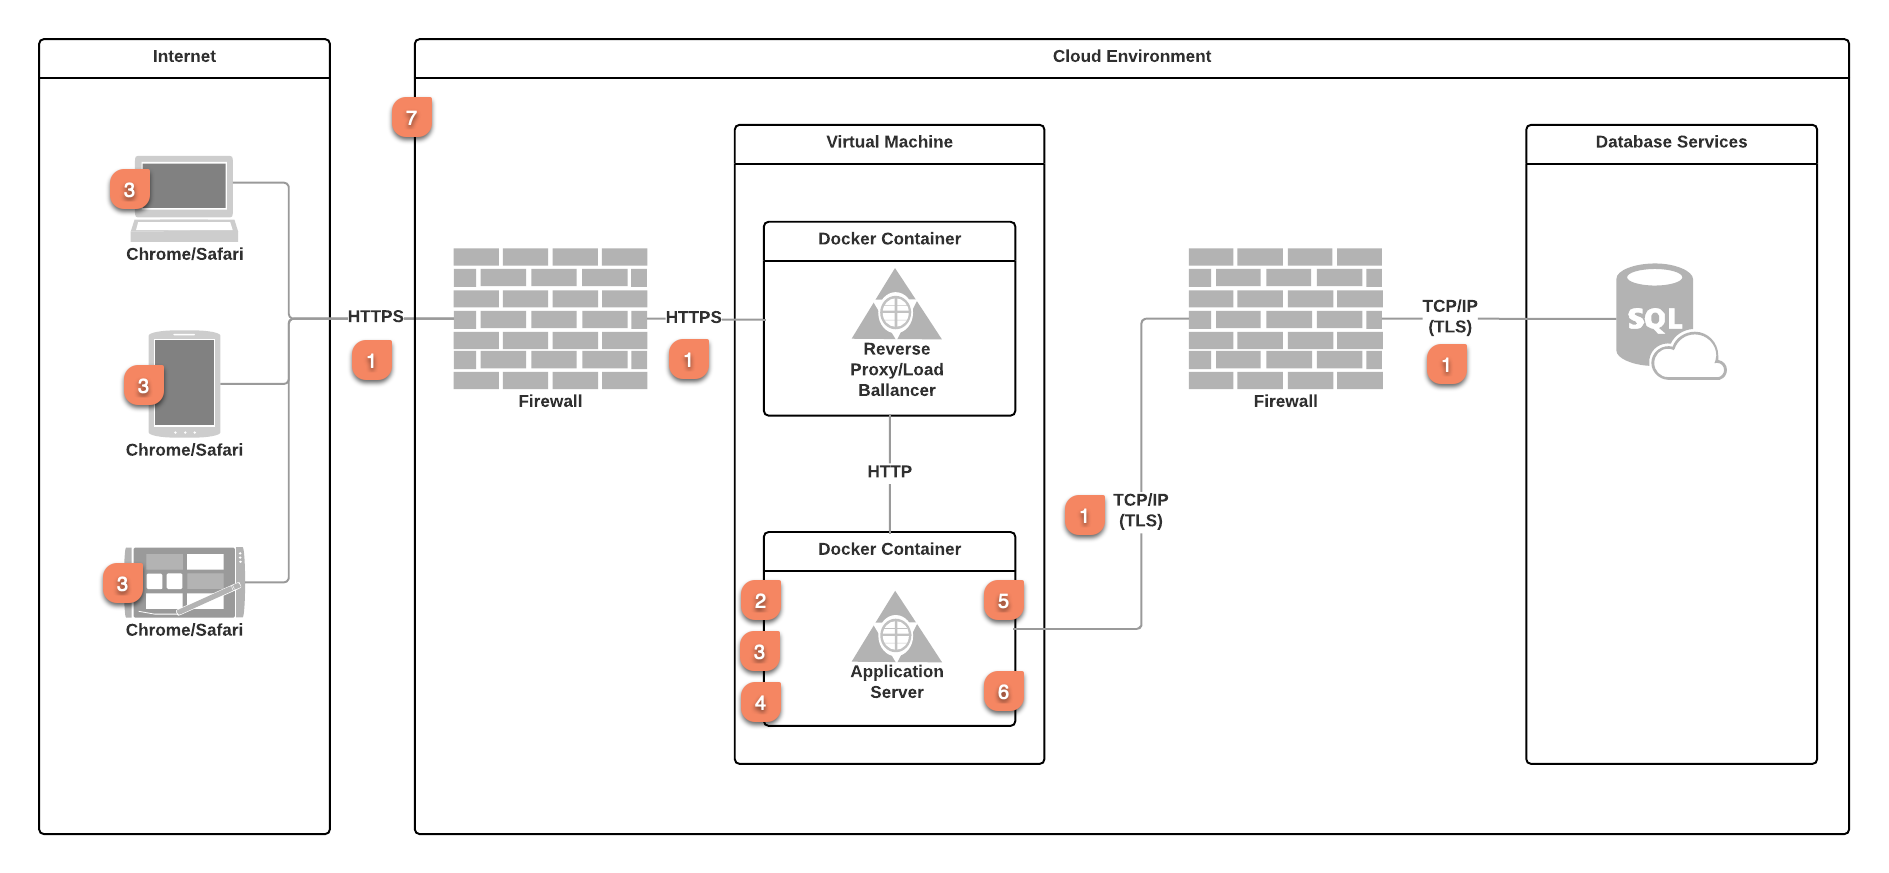
\includegraphics[width=1\linewidth]{images/01-security-diagram.png}
	\caption{A high-level security diagram for TG applications.}\label{sec:01:fig:1}
	\end{figure}

\section*{Authentication}

\subsection*{Server Authentication for User Protection}

\subsubsection*{How HTTPS works}

\subsubsection*{Communication over HTTPS}

\subsection*{Client Authentication for Server Protection}

\subsubsection*{Login and 2-factor authentication}

\paragraph*{Password strength}

\paragraph*{Preventing rapid-fire login attempts}

\subsubsection*{Restoring a password}


\subsubsection*{Reduced Sign-On instead of Single Sign-On}

\paragraph*{Authenticators}


\section*{Authorisation}

\subsection*{User roles and security tokens}

\paragraph{Security Matrix.}

\section*{User-driven data filtering}

\section*{Deployment environment and its security}

%
% ---- Bibliography ----
%
\begin{thebibliography}{5}

\bibitem{Kay2003}
Kay, A. On the Meaning of ``Object-Oriented Programming''
\href{http://www.purl.org/stefan_ram/pub/doc_kay_oop_en}{Online}

\bibitem{Barnes:2007:ORM}
Bar\-nes, J.~M. Object-Relational Mapping as a Persistence Mechanism for Object-Oriented Applications, 2007,
\href{http://digitalcommons.macalester.edu/mathcs_honors/6/}{Online}

\bibitem{DeMichiel:2012:JPA}
De\-Mi\-chiel. L. JSR 338: Java Persistence API, Version 2.1, 2012,
\href{http://jcp.org/aboutJava/communityprocess/pr/jsr338/index.html}{Online}

\bibitem{evans2003}
Evans, E. Domain-Driven Design: Tackling Complexity in the Heart of Software, 2003, Addison-Wesley Professional.

\bibitem{Fowler:2010:DSL}
Fow\-ler, M. Domain-Specific Languages, Addison-Wesley Professional, 2010.

\bibitem{Fowler:2012:OH}
Fow\-ler. M. OrmHate, 2012,
\href{http://martinfowler.com/bliki/OrmHate.html}{Online}

\bibitem{Fielding2000}
Fielding, R. T. Architectural styles and the design of network-based software architectures: Phd thesis, University of California, Irvine, USA, 2000.

\bibitem{HBBPB:2008}
Hambrick, G. et al. Persistence in the Enterprise: A Guide to Persistence Technologies, 2008, IBM Press.

\bibitem{haywood2009}
Haywood, D. Domain-Driven Design Using Naked Objects, 2009, Pragmatic Bookshelf.

\bibitem{Hodych:2012}
Hodych, O. et al. Visual Domain-Specific Query Language for Business Applications, in Proceedings of 14-th International Conference on System Analysis and Information Technologies (SAIT 2012), Kyiv, Ukraine, 2012, pp. 311-312.

\bibitem{Hodych:2013}
Hodych, O. et al. Object-relational mapping: Limitations of data querying, in Proceedings of 15-th International Conference on System Analysis and Information Technologies (SAIT 2013), Kyiv, Ukraine, May 27-31, 2013. — P. 376–377.

\bibitem{HHN1986}
Hutchins, E., Holland, J. and Norman, D. Direct Manipulation Interfaces, in User Centered System Design: New Perspectives on Human-computer Interaction, 1986, CRC Press.

\bibitem{jacobson1992}
Jacobson, I. Object Oriented Software Engineering: A Use Case Driven Approach, 1992, Addison-Wesley Professional.

\bibitem{UBob:2002}
Martin, R.~C. Agile Software Development, Principles, Patterns, and Practices, 2002, Prentice Hall.

\bibitem{Neward:2006:VCS}
New\-ard. T. The Vietnam of Computer Science, 2006,
\href{http://blogs.tedneward.com/2006/06/26/The+Vietnam+Of+Computer+Science.aspx}{Online}

\bibitem{oli2007}
Oliv\'{e}, A. Conceptual Modeling of Information Systems, 2007, Springer.

\bibitem{pawson2001}
Pawson, R. and Matthews, R. Naked objects: a technique for designing more expressive systems, SIGPLAN Notices, V.36(12), pp.61--67, 2001.

\bibitem{pawson2004}
Pawson, R., Naked Objects, Ph.D Thesis, 2004, Trinity College, Dublin, Ireland.

\bibitem{vernon2013}
Vernon, V. Implementing Domain-Driven Design, 2013, Addison-Wesley Professional.

\bibitem{shneiderman1982}
Shneiderman, B. The future of interactive systems and the emergence of direct manipulation. Behaviour and Information Technology, 1(3):237–256, 1982.

\bibitem{shneiderman1983}
Shneiderman, B. Direct manipulation: A step beyond programming languages. Computer, 16(8):57–69, 1983.

\bibitem{fowler2003} Fowler, M. AnemicDomainModel, 
\href{http://www.martinfowler.com/bliki/AnemicDomainModel.html}{Online}

\bibitem{fowler2006} Fowler, M. DslBoundary, 
\href{http://martinfowler.com/bliki/DslBoundary.html}{Online}

\bibitem{bozhanov2010} Bozhanov, B. On Domain-Driven Design, Anemic Domain Model, Code Generation, Dependency Injection and More…
\href{http://techblog.bozho.net/on-domain-driven-design-anemic-domain-models-code-generation-dependency-injection-and-more/}{Online}

\bibitem{sapm2014}  The Anaemic Domain Model is no Anti-Pattern, it’s a SOLID design, The School of Informatics, University of Edinburgh,
\href{https://blog.inf.ed.ac.uk/sapm/2014/02/04/the-anaemic-domain-model-is-no-anti-pattern-its-a-solid-design/}{Online}

\bibitem{yegge2006} Yegge, S. Execution in the Kingdom of Nouns,  
\href{http://steve-yegge.blogspot.com.au/2006/03/execution-in-kingdom-of-nouns.html}{Online}

\bibitem{SOLID} SOLID (object-oriented design), 
\href{https://en.wikipedia.org/wiki/SOLID_(object-oriented_design)}{Online}

\bibitem{CQRS} CQRS design pattern, 
\href{https://cqrs.files.wordpress.com/2010/11/cqrs_documents.pdf}{Online}

\end{thebibliography}
%

\end{document}

